\subsubsection{Creation of a Report}
Whenever the user wants to send a report of a parking violations to the authorities he has to follow what is visually described in the diagram below.
The user needs to insert a set of photos where a license plate is readable, and after confirming that the app has successfully read the license plate of the vehicles in the photos he should complete the form with the information required. At last he has to select if he wants to send an automatic or a manual ticket to the officers, after that the process is completed.
\\\\\\\\
\makebox[\textwidth][c]{
	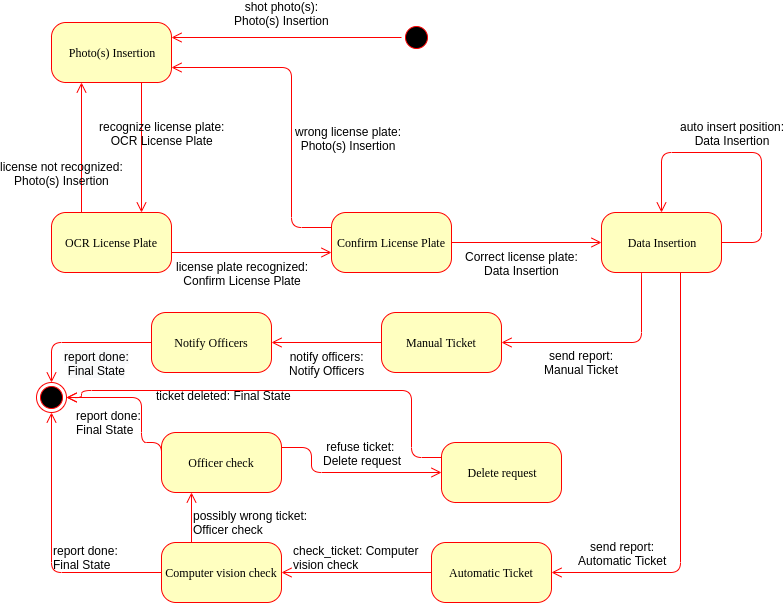
\includegraphics[width=1.2\textwidth]{diagrams/images/creationOfAReport}
}
\clearpage
\subsubsection{Statistics Construction}
At the end of the day the statistics need to be updated in order to offer to the users and to the officers only recent, and therefore consistent, information.
When the servers will probably have the lowest load, so in the middle of the night, SafeStreets will at first retrieve the new data that are now present in both the reports DB and the accidents DB. Once the complex queries have returned the new information the data needs to be aggregate and elaborate in order to exhibit the updated statistics to the costumers of SafeStreets. 
\\\\\\\\
\makebox[\textwidth][c]{
	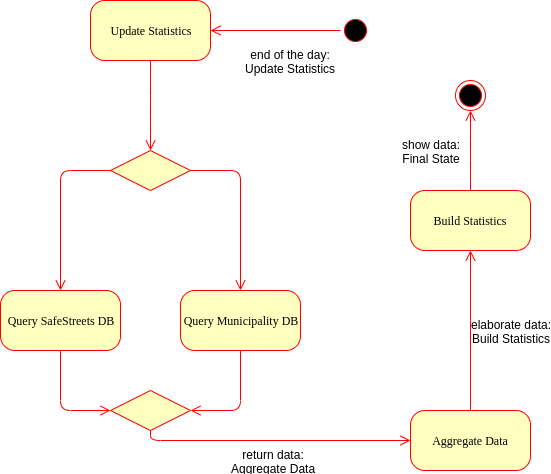
\includegraphics[width=\textwidth]{diagrams/images/statisticsConstruction}
}
\clearpage
\subsubsection{Data mining for Suggestions}
\clearpage
\subsubsection{Basic UX}
\clearpage